% --------------------------------------------------------------------------- %
% Poster for the SSC 2012 Conference (Case Study).      %
% --------------------------------------------------------------------------- %
% Created with Brian Amberg's LaTeX Poster Template. Please refer for the     %
% attached README.md file for the details how to compile with `pdflatex`.     %
% --------------------------------------------------------------------------- %
% $LastChangedDate:: 2011-09-11 10:57:12 +0200 (V, 11 szept. 2011)          $ %
% $LastChangedRevision:: 128                                                $ %
% $LastChangedBy:: rlegendi                                                 $ %
% $Id:: poster.tex 128 2011-09-11 08:57:12Z rlegendi                        $ %
% --------------------------------------------------------------------------- %
\documentclass[paperwidth=58in,paperheight=47in,portrait]{baposter}

\usepackage{relsize}		% For \smaller
\usepackage{url}			% For \url
\usepackage{epstopdf}	% Included EPS files automatically converted to PDF to include with pdflatex
\usepackage{array}
\usepackage{multicol}
\usepackage{lmodern}
\usepackage[T1]{fontenc}

%\setlength{\columnseprule}{1pt}

\def\thousandseparator{,}

%%% Global Settings %%%%%%%%%%%%%%%%%%%%%%%%%%%%%%%%%%%%%%%%%%%%%%%%%%%%%%%%%%%

\graphicspath{{pix/}}	% Root directory of the pictures 
\tracingstats=2			% Enabled LaTeX logging with conditionals

%%% Color Definitions %%%%%%%%%%%%%%%%%%%%%%%%%%%%%%%%%%%%%%%%%%%%%%%%%%%%%%%%%

\definecolor{bordercol}{RGB}{0,0,0}
\definecolor{headercol1}{RGB}{106,0,255}
\definecolor{headercol2}{RGB}{106,0,255}
\definecolor{headerfontcol}{RGB}{255,255,255}
\definecolor{boxcolor}{RGB}{255,255,255}
\definecolor{backcolor1}{RGB}{216,255,150}
\definecolor{backcolor2}{RGB}{216,255,150}
\definecolor{titlecol}{RGB}{0,0,0}


%%%%%%%%%%%%%%%%%%%%%%%%%%%%%%%%%%%%%%%%%%%%%%%%%%%%%%%%%%%%%%%%%%%%%%%%%%%%%%%%
%%% Utility functions %%%%%%%%%%%%%%%%%%%%%%%%%%%%%%%%%%%%%%%%%%%%%%%%%%%%%%%%%%

%%% Save space in lists. Use this after the opening of the list %%%%%%%%%%%%%%%%
\newcommand{\compresslist}{
	\setlength{\itemsep}{1pt}
	\setlength{\parskip}{0pt}
	\setlength{\parsep}{0pt}
}

%%%%%%%%%%%%%%%%%%%%%%%%%%%%%%%%%%%%%%%%%%%%%%%%%%%%%%%%%%%%%%%%%%%%%%%%%%%%%%%
%%% Document Start %%%%%%%%%%%%%%%%%%%%%%%%%%%%%%%%%%%%%%%%%%%%%%%%%%%%%%%%%%%%
%%%%%%%%%%%%%%%%%%%%%%%%%%%%%%%%%%%%%%%%%%%%%%%%%%%%%%%%%%%%%%%%%%%%%%%%%%%%%%%

\global\hyphenpenalty=100000

\begin{document}
\typeout{Poster rendering started}

%%% Setting Background Image %%%%%%%%%%%%%%%%%%%%%%%%%%%%%%%%%%%%%%%%%%%%%%%%%%
%\background{
%	\begin{tikzpicture}[remember picture,overlay]%
%	\draw (current page.north west)+(-2em,2em) node[anchor=north west]
%	{
\includegraphics[height=1.1\textheight]{background}};
%	\end{tikzpicture}
%}

%%% General Poster Settings %%%%%%%%%%%%%%%%%%%%%%%%%%%%%%%%%%%%%%%%%%%%%%%%%%%
%%%%%% Eye Catcher, Title, Authors and University Images %%%%%%%%%%%%%%%%%%%%%%
\begin{poster}{
	grid=false,
	% Option is left on true though the eyecatcher is not used. The reason is
	% that we have a bit nicer looking title and author formatting in the headercol
	% this way
	eyecatcher=true, 
	borderColor=bordercol,
	headerColorOne=headercol1,
	headerColorTwo=headercol2,
	headerFontColor=headerfontcol,
	% Only simple background color used, no shading, so boxColorTwo isn't necessary
	boxColorOne=boxcolor,
	headershape=rounded,
	headerfont=\Large\sf\bf,
	textborder=rounded,
	background=shadetb,
	bgColorOne=backcolor1,
	bgColorTwo=backcolor2,
	headerborder=closed,
  boxshade=plain,
  columns=4
}
%%% Eye Cacther %%%%%%%%%%%%%%%%%%%%%%%%%%%%%%%%%%%%%%%%%%%%%%%%%%%%%%%%%%%%%%%
{
%\setlength\fboxsep{0pt}
%\setlength\fboxrule{0.5pt}
%	\fbox{
%		\begin{minipage}{14em}
			%\includegraphics[width=14em]{SFU.png}
			
\includegraphics[width=14em]{UFV.png}
%			
\includegraphics[width=4em,height=4em]{elte_logo} \\
%			
\includegraphics[width=10em,height=4em]{dynanets_logo}
%			
\includegraphics[width=4em,height=4em]{aitia_logo}
%		\end{minipage}
%	}
}
%%% Title %%%%%%%%%%%%%%%%%%%%%%%%%%%%%%%%%%%%%%%%%%%%%%%%%%%%%%%%%%%%%%%%%%%%%
{\sf\bf
	\color{titlecol}Investigating the Effect of Design Weights in a Complex Survey Design
}
%%% Authors %%%%%%%%%%%%%%%%%%%%%%%%%%%%%%%%%%%%%%%%%%%%%%%%%%%%%%%%%%%%%%%%%%%
{
	\vspace{1em} Jonathan Fitz and Dong Liang, University of the Fraser Valley\\
	{\smaller Jonathan.Fitz@student.ufv.ca, Dong.Liang@student.ufv.ca}
}
%%% Logo %%%%%%%%%%%%%%%%%%%%%%%%%%%%%%%%%%%%%%%%%%%%%%%%%%%%%%%%%%%%%%%%%%%%%%
{
% The logos are compressed a bit into a simple box to make them smaller on the result
% (Wasn't able to find any bigger of them.)
%\setlength\fboxsep{0pt}
%\setlength\fboxrule{0.5pt}
%	\fbox{
%		\begin{minipage}{14em}
			%\includegraphics[width=14em]{SFU.png}
			
\includegraphics[width=14em]{ufv.jpg}
%			
\includegraphics[width=4em,height=4em]{elte_logo} \\
%			
\includegraphics[width=10em,height=4em]{dynanets_logo}
%%			
\includegraphics[width=4em,height=4em]{aitia_logo}
%		\end{minipage}
%	}
}


\headerbox{Introduction}{name=Introduction,column=0,row=0}{
\textbf{Objective}:  Determine the risk factors for hypertension among Canadians with and without design weights. Investigate whether these risk factors depend on gender or age.\\

\textbf{Study}: Statistics Canada conducted Cycle 3 of their Canadian Health Measures Survey from 2012-2013, a survey that utilizes two different kinds of weights.
\begin{itemize}
\item A Mobile Examination Centre (MEC) was used to take direct physical measurements from approximately 3000 Canadians across the ten provinces.
\item Survey weights were assigned to each study participant to insure that the sample represented the target population.
\item Due to the complexity of the stratified three-stage sample design, bootstrap weights were created to estimate the variance of estimators.
%\item These 500 bootstrap weights were used to create 500 estimates, and the variance of the estimate was estimated with the variance of these 500 bootstrap weights.
\end{itemize}

\textbf{Response}: HIGHBP: Categorized hypertensive: 1 yes, 2 no.  \\

\textbf{Potential Risk Factors}: The following measurements were taken directly from study participants using the MEC:
\begin{itemize}
\item SMK: Smoking status: 1 daily; 2 occasional; 3 non-smoker.
\item SEX: Sex at clinic visit: 1 male, 2 female.
\item AGE: Age in years at clinic visit: 20 to 79.
\item BMI: Body mass index in kg/m2. 
\item BCD: Blood cadmium in nmol/L. 
\item BHG: Blood mercury in nmol/L.
\end{itemize}
}





\headerbox{Notation}{name=Notation,column=0,below=Introduction}{
\textbf{Data}: Let $i$ denote the study participant, and $j$ the explanatory variable. Other useful terms are defined below:
\begin{itemize}
\item $y$: Vector whose $i$th element is the HIGHBP value of the $i$th study participant.
\item $X$: Design matrix whose $ij$th element is the observed value of the $j$th covariate for the $i$th study participant.
\item $w$: Vector whose $i$th element is the survey or bootstrap weight for the $i$th study participant .
%\end{itemize}
%\textbf{Parameters}:
%\begin{itemize}
\item $n$, $V$: Sample size and variance respectively.
\item $f(X)$: The probability mass function for HIGHBP.
\item $\mu$: Vector whose $i$th element equals the expected value of HIGHBP for the $i$th study participant.
\item $\beta$: Vector whose $j$th element is the coefficient of the $j$th explanatory variable.
\item $g(\mu)$: Link function to model the relationship between $\mu$ and the explanatory variables.
\item $q$: Number of parameters set to zero in null hypothesis.
\end{itemize}
}



\headerbox{Cleaning the Data}{name=Imputation,column=0,span=1, below=Notation}{
\textbf{Censored Data}: The variables BCD and BHG both contained data that was below their respective Limit of Detection (LOD).
\begin{itemize}
\item This censored data was imputed with values randomly drawn from the interval [0, LOD].
\item Popular alternatives include imputing using a single value such as LOD or LOD/2, but our approach should better account for the variance of the true (unknown) data.
\end{itemize}
}



\headerbox{Cleaning the Data Continued}{name=Imputation2,column=1,span=1, row=0}{
\textbf{Missing Data}: Roughly $6\%$ of observations across four variables contained missing data.
\begin{itemize}
\item This missing data was imputed using K-nearest neighbors (KNN), and 5-fold cross-validation was used to pick K.
\item Four KNN models were built, each having as the response one of the four variables with missing data.
\item The training set for these models was the set of all observations that did not contain any missing data.
\end{itemize}

}





\headerbox{Models}{name=Model,column=1,span=1, below=Imputation2}{
\textbf{Unweighted Model Estimators}: A generalized linear model without using design weights was first fitted.
\begin{itemize}
\item HIGHBP was modelled as binary response r.v.'s with parameters $\mu$, and the logit was chosen for the link function.
\end{itemize}
The model coefficients $\beta$ were estimated using maximum likelihood, which satisfy the following equation:

\begin{equation}
% This equation is supposed to equal the equation right before (3.1) in the paper "Fitting Regression Models to Survey Data" on github
U(\hat{\beta}) = \sum_{i=1}^n x_{i}\frac{1}{g'(\mu_{i})V(\mu_{i})}\left(y_{i} - \mu_{i}(\hat{\beta})\right) = 0
\end{equation}


\textbf{Weighted Model Estimators}: Following Lumley and Scott (2017), the score function above was altered to incorporate design weights:

\begin{equation}
% This equation is supposed to equal (3.1) in the paper "Fitting Regression Models to Survey Data" on github (without R_i, since we use sample size n instead of population size N)
U(\hat{\beta}) = \sum_{i=1}^n w_{i}x_{i}\frac{1}{g'(\mu_{i})V(\mu_{i})}\left(y_{i} - \mu_{i}(\hat{\beta})\right) = 0
\end{equation}


\textbf{Estimating Variance}: 
\begin{itemize}
\item For unweighted model, the variance of model coefficients were estimated using the inverse of the Information matrix.
\item For weighted model, each of the 500 bootstrap weights was used with (2) to calculate 500 more estimates. The variance of these estimates was the estimated variance of the model coefficients.
\end{itemize}
}






\headerbox{Exploratory Analysis}{name=EDA,column=1,below=Model}{
\textbf{EDA}: Plots were made to understand the structure of the data.
\begin{itemize}
\item Continuous variables were plotted as categorical to avoid observed hypertension proportions of 0 or 1.
\item Since the explanatory variables exhibit low linear correlation, we can make useful plots without holding all other variables constant.
\end{itemize}

\begin{multicols}{2}
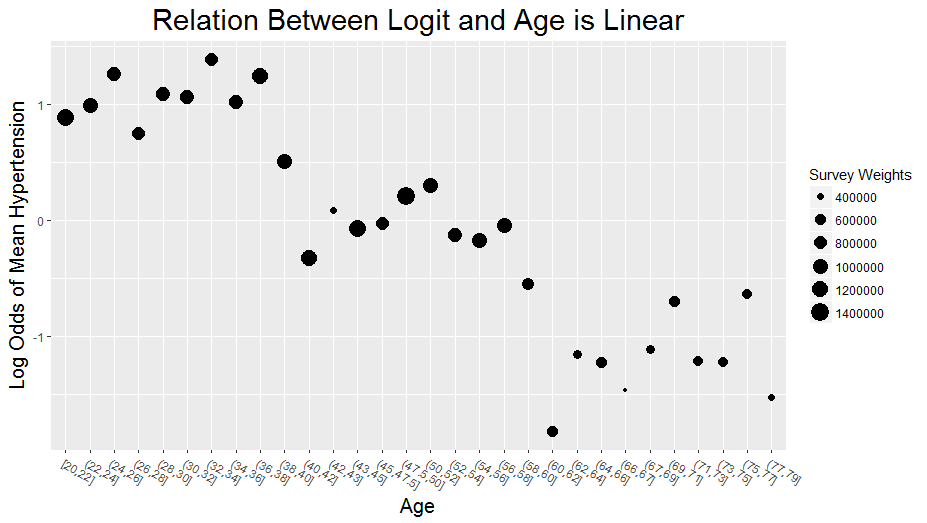
\includegraphics[width=14em]{Logit_Age.png}\\
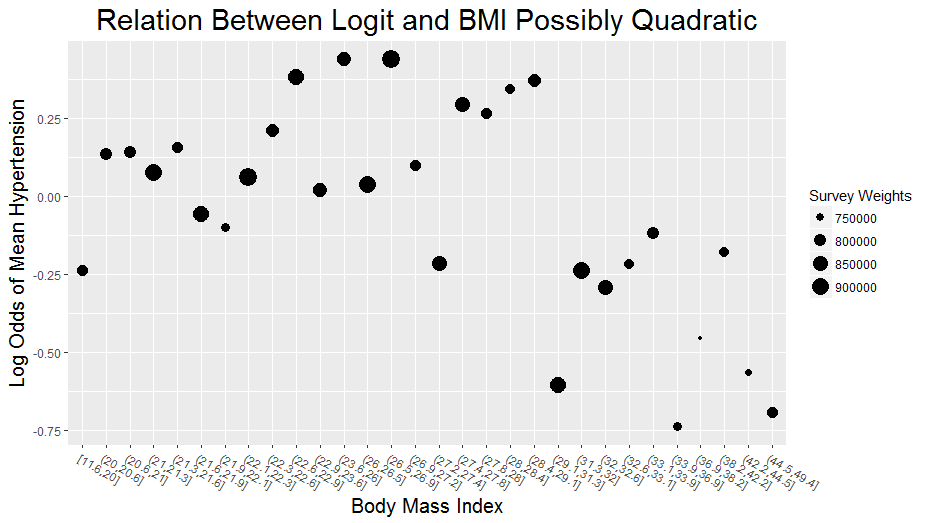
\includegraphics[width=14em]{Logit_BMI.png}
\end{multicols}




\begin{multicols}{2}
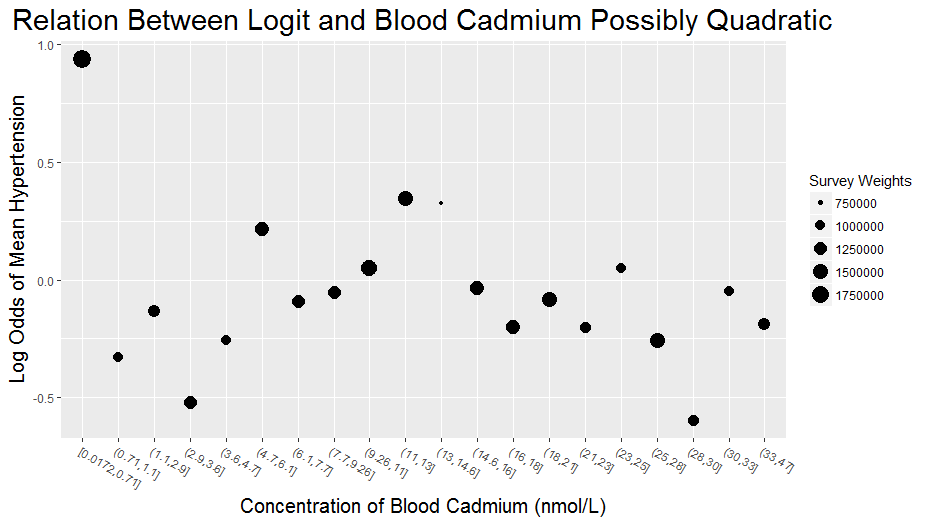
\includegraphics[width=14em]{Logit_Cadmium.png}\\
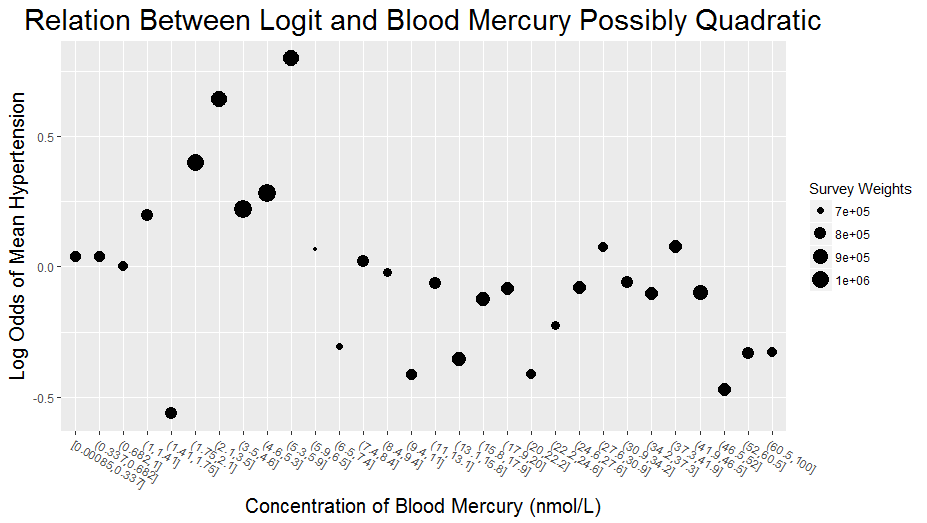
\includegraphics[width=14em]{Logit_Mercury.png}
\end{multicols}

\textbf{Conclusion}: Including second-order terms for BMI, BCD, and BHG in the model could be informative, but isn't necessary for AGE.

% Say something about how BIC also justifies this choice...
}



\headerbox{Checking Model Fit}{name=fit,column=2,row=0}{
%Checking the variance inflation factors (VIF) confirmed that multicollinearity was not a problem.
\textbf{Goodness of Fit}: Since the response is binary, the Hosmer-Lemeshow test statistic was used to check overall goodness of fit.
\begin{itemize}
\item Follows $\chi_{g-2}^2$ under null hypothesis that model fits sample data well (Hosmer et al., 1980).
\item No theoretical guidance for choosing g, so we chose several values and used the average p-value.
\end{itemize}
}



\headerbox{Hypothesis Testing Theory}{name=Testing,column=2,below=fit}{
\textbf{Null Hypothesis}: Suppose $\beta$ is partitioned by ($\beta_{(1)}$, $\beta_{(2)}$). The null hypothesis is $H_{0}$: $\beta_{(1)}$ = 0, where $\beta_{(1)}$ has dimension $q$. \\

\textbf{Unweighted Model}: For the unweighted model, the log-likelihood ratio statistic under $H_{0}$ follows $\chi_{q}^2$. \\

\textbf{Weighted Model}: The likelihood functions do not exist for the weighted model. Following Lumley $\&$ Scott, 2017, the unweighted likelihood formulas were altered to include weights:

\begin{equation}
% This should equal the equation right before (4.1) in the paper "Fitting Regression Models to Survey Data" on github
\ell(\beta) = \sum_{i=1}^n w_{i}\log{f(y_{i}|x_{i}; \beta)}
\end{equation}

The "working likelihood ratio test statistic" was then defined as 

\begin{equation}
% This should equal the equation (4.1) in the paper "Fitting Regression Models to Survey Data" on github
\tau = 2\left[\ell(\hat{\beta}) - \ell(\hat{\beta^*}) \right]
\end{equation}

where $\hat{\beta^*}$ is the solution to (3) when $\beta_{(1)}$ = 0.
The saddlepoint approximation (Kuonen, 1999)  was used to approximate the distribution of $\tau$.

%\textbf{Special Case}: If response is binary and q is not small, then log-likelihood statistic will not follow $\chi_{q}^2$ (Dobson $\&$ Barnett 2008).
%\begin{itemize}
%\item The Hosmer-Lemeshow test statistic follows $\chi_{g-2}^2$ under the null hypothesis that the proposed model fits as well as the saturated model
%
%\end{itemize}
}






\headerbox{Results}{name=Results,column=2,span=1, below=Testing}{
\textbf{Model Without Interactions}: Hypothesis testing on both the unweighted and weighted model without interaction effects was carried out.

\begin{center}
\scalebox{0.9}{\begin{tabular}{r|c|c|c}
       Null &     $ p$ (Unweighted) &          $p$ (Weighted) &      Design Effects \\ \hline
       SMK 2 = 0 &		0.113 &				0.472 &			     0.882 \\
       SMK 3 = 0 &				&					&			     0.948 \\  \hline	
       SEX = 0 &			 \textcolor{red}{0.001} &  \textcolor{red}{0.005} &		     1.14  \\  \hline
       AGE = 0 &			 \textcolor{red}{0.000}&\textcolor{red}{0.000}&		     1.06  \\  \hline
       BMI = 0 &			 \textcolor{red}{0.000}&	 \textcolor{red}{0.002}&		     1.50  \\
      $ \mathrm{BMI}^2$ = 0 & 				&					&			     1.55 \\  \hline
       BCD = 0 &			0.505 &				0.731 &  			     1.59  \\
       $\mathrm{BCD}^2$ = 0 &				&					&		    	     1.66 \\  \hline
       BHG = 0&			 \textcolor{red}{0.048}&				0.185&			     1.38 \\
       $\mathrm{BHG}^2$ = 0 &				&					&			     1.43 \\  \hline
\end{tabular}}
\end{center}

\begin{itemize}
\item Very strong evidence (p-value < 0.01) that AGE , SEX, and BMI for both unweighted and weighted models affect mean HIGHBP, when other risk factors are accounted for.
\item Some evidence (0.01 < p-value < 0.05) that BHG affects mean HIGHBP, but only for unweighted model.
\item Little to no evidence that other variables affect mean HIGHBP when other risk factors are accounted for.
\end{itemize}

\textbf{Model with Interactions}: Three interaction effects are now added to both the unweighted and weighted model.
\begin{center}
\scalebox{0.9}{\begin{tabular}{r|c|c|c}
       Null&    $p$ (Unweighted) &       $p$ (Weighted) &      Design Effects \\ \hline
       SEX:AGE= 0 &			0.143 &				 \textcolor{red}{0.048} &				0.869 \\  \hline
       SEX:BMI = 0 &			 \textcolor{red}{0.046} &				0.093 &				1.41 \\  \hline
       AGE:BMI = 0 &			0.149 &				 \textcolor{red}{0.046}&				1.16 \\  \hline
\end{tabular}}
\end{center}

\begin{itemize}
\item For unweighted model, some evidence (p-value < 0.05) that effect of BMI on HIGHBP depends on SEX.
\item For weighted model, some evidence (p-value < 0.05) that effects of SEX and BMI on HIGHBP depend on AGE.
\item Little to no evidence that other variables affect mean HIGHBP when other risk factors are accounted for.
\end{itemize}
}


\headerbox{Results Continued}{name=Results Continued,column=3,span=1,row=0} {
\textbf{Analysis}: Odds Ratio plots can clarify these interaction effects.

\begin{multicols}{2}
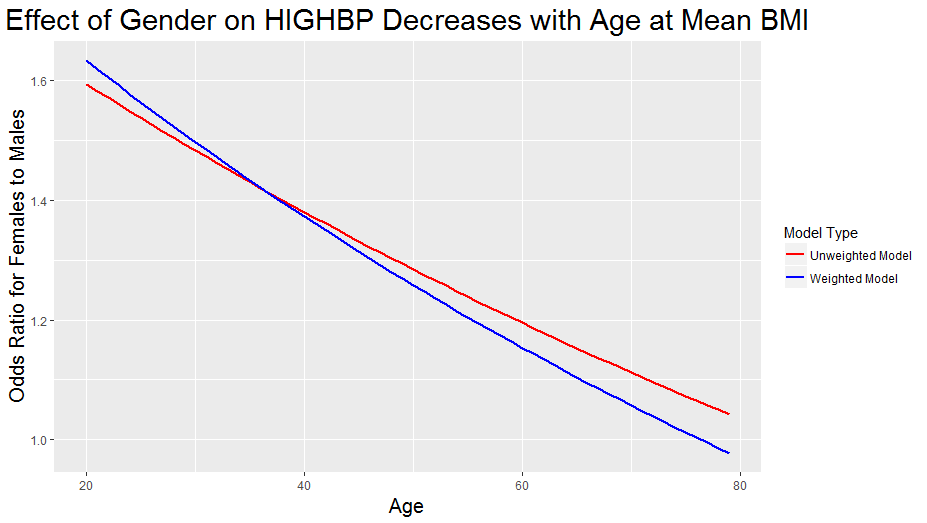
\includegraphics[width=14em]{SexOdds_Age.png} \\
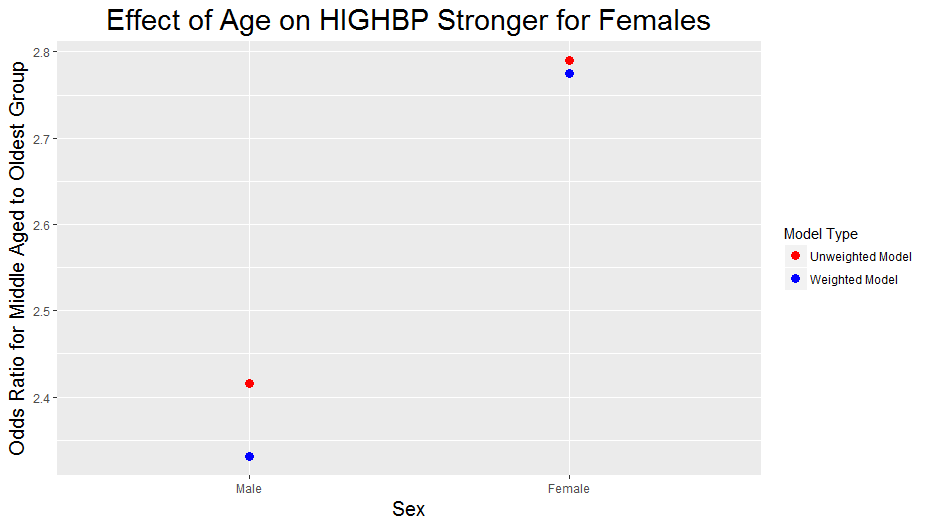
\includegraphics[width=14em]{AgeOdds_Sex.png} 
\end{multicols}

\begin{itemize}
\item At older ages, SEX is a weaker risk factor (predictor) for HIGHBP, when other variables are fixed.
\item For females, AGE is a stronger risk factor for HIGHBP
\end{itemize}

\begin{multicols}{2}
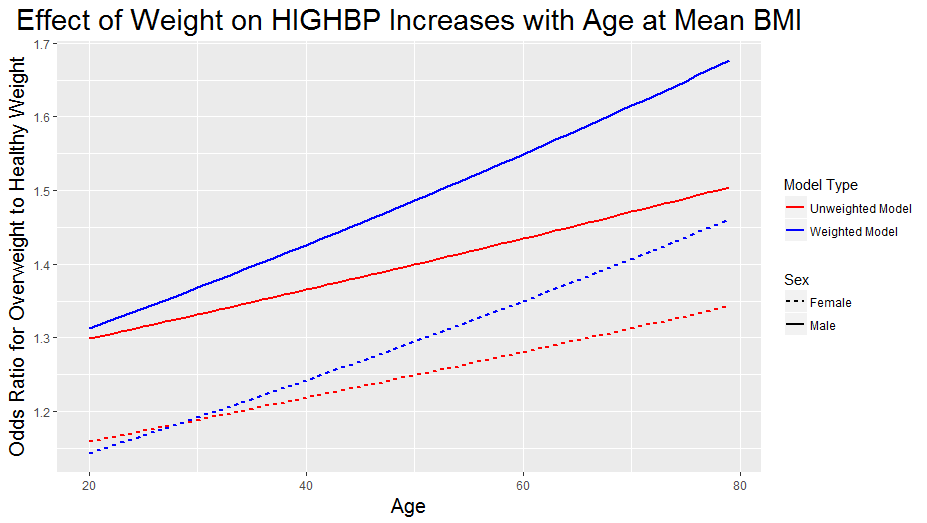
\includegraphics[width=14em]{WeightOdds_Age.png} \\
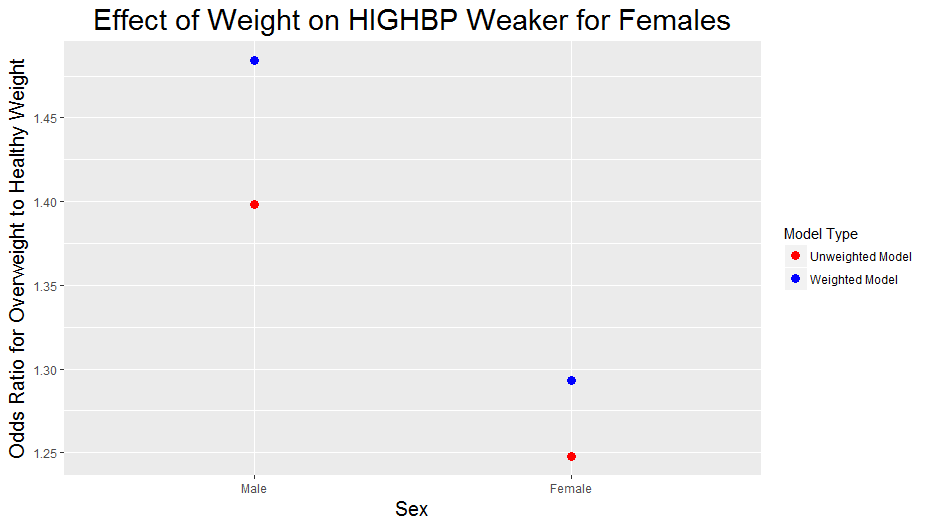
\includegraphics[width=14em]{WeightOdds_Sex.png} 
\end{multicols}

\begin{itemize}
\item At older ages, BMI is a stronger risk factor for HIGHBP.
\item For males, BMI is a stronger risk factor for HIGHBP.
\end{itemize}

Keep in mind that only for certain models (see interaction p-values) is there some evidence of these interaction effects. \\

\textbf{Design Effects}: For an estimator, the design effect is the ratio of weighted variance to unweighted variance. This makes it easy to see that BCD, BMI, BHG, and SEX:BMI have weighted variances that are quite different from their unweighted variances.
}






\headerbox{Further Work}{name=further,column=3,below=Results Continued}{
\textbf{Weighted Model Fit}: The weighted model was not checked for model fit. A goodness of fit test that can take weights into account was suggested by Archer et al., 2007.  \\\\
\textbf{Variance of Imputation}: The uncertainty in the imputed censored and missing data was ignored, and this will artificially deflate the variance of the estimators. Can use a method such as the bootstrap to estimate the error introduced by this imputation. \\\\
\textbf{Improved Imputation}: Use a more sophisticated method such as survival analysis to estimate the censored data. 
}


\headerbox{References}{name=references,column=3,span=1, below=further}{
\smaller
\begin{itemize}
%\item Dobson, A. J., \& Barnett, A. G. (2008). \emph{An introduction to generalized linear models.} Boca Raton: CRC Press, Taylor \& %Francis Group.
\item Archer, K. J., Lemeshow, S., \& Hosmer, D. W. (2007). Goodness-of-fit tests for logistic regression models when data are collected using a complex sampling design. \emph{Computational Statistics \& Data Analysis}, 51(9), 4450-4464. doi:10.1016/j.csda.2006.07.006.
\item Hosmer, D. W. \& S. Lemeshow (1980). Goodness of fit tests for the multiple logistic model. \emph{Communications in Statistics-Theory and Methods} A9, 1043-1069.
\item Kuonen, D. (1999). \emph{Saddlepoint approximations for distributions of quadratic forms in normal variables.} Biometrika 86 929-935.
%\item Lumley, T. (2010).  \emph{Complex surveys: A guide to analysis using R.} Hoboken, NJ: John Wiley.
\item Lumley, T., \& Scott, A. (2017). Fitting Regression Models to Survey Data. \emph{Statistical Science}, 32(2), 265-278. doi:10.1214/16-STS605.
\end{itemize}
}



\headerbox{Acknowledgements}{name=acknowledgements,column=3,below=references}{
\smaller						% Make the whole text smaller
%\vspace{-0.4em}			% Save some space at the beginning
We are very grateful to Shaun Sun, whose guidance and technical expertise made this project possible. We also thank Thomas Lumley for making public his R survey() package that was used extensively in this analysis.
} 

\end{poster}
\end{document}